% DriftLens -- Springer LNCS format (llncs class, splncs04 bibliography style)
% Compile: pdflatex driftlens_lncs && bibtex driftlens_lncs && pdflatex driftlens_lncs && pdflatex driftlens_lncs
\documentclass[runningheads]{llncs}

\usepackage[T1]{fontenc}
\usepackage{lmodern}
\usepackage{graphicx}
\usepackage{booktabs}
\usepackage{array}
\usepackage{amsmath,amssymb}
\usepackage{multirow}
\usepackage{xcolor}
\usepackage{tikz}
\usetikzlibrary{arrows.meta,positioning,fit}
\usepackage[hidelinks]{hyperref}
\usepackage{url}

\graphicspath{{../results/figures/}}
\newcommand{\state}[1]{\textsc{#1}}

\begin{document}

\title{DriftLens: Reading a Social-Media Timeline as a Sentence to Detect Moments of Change with Classical NLP}
\titlerunning{DriftLens: Moments of Change with Classical NLP}

% Three author columns; replace [email] with the co-authors' addresses.
\author{%
\begin{tabular}{@{}>{\centering\arraybackslash}p{0.31\textwidth}>{\centering\arraybackslash}p{0.31\textwidth}>{\centering\arraybackslash}p{0.31\textwidth}@{}}
B Varun & Sagnik Basu & Arivoli A \\[3pt]
\small Vellore Institute of Technology, Vellore, India &
\small Vellore Institute of Technology, Vellore, India &
\small Vellore Institute of Technology, Vellore, India \\[2pt]
\small\texttt{varun452005@gmail.com} & \small\texttt{[email]} & \small\texttt{[email]}
\end{tabular}}
\authorrunning{B Varun et al.}
\institute{}

\maketitle

\begin{abstract}
People who write about their mental health online rarely change in one step. Some posts mark a sudden shift in mood, while others belong to a slow slide or a slow recovery. We ask how far the classical NLP toolkit can go in finding these moments of change, without large language models. DriftLens reads a user's timeline the way a part-of-speech tagger reads a sentence: each post receives a hidden state (no change, switch, escalation, or both) decoded with hidden Markov models or conditional random fields. The per-post evidence comes from components that we build and evaluate one by one: a noisy-channel spelling corrector, a WordNet-grown self-state lexicon with sense filtering and adapted Lesk disambiguation, an HMM tagger that feeds a grammar for self-evaluative statements, and a personal language-model score of how unlike their own history a user sounds. On the 30 labelled CLPsych timelines (373 posts), the sequence models reach a macro-F1 of 0.567 against 0.266 for the majority baseline, and they detect escalation better than a per-post maximum-entropy classifier. A single feature, post length, already gives 0.572, and we treat this shortcut as a finding rather than hide it: within posts of similar length the linguistic features add 0.09 to 0.13 macro-F1 over the length model. The lexicon tracks annotated well-being better than VADER (Spearman $\rho$ 0.43 vs.\ 0.36) and, with no training labels, separates depressed from control users in eRisk 2026 with an AUC of 0.84.

\keywords{Moments of change \and Sequence labelling \and Hidden Markov models \and WordNet \and N-gram language models \and Mental health}
\end{abstract}

%======================================================================
\section{Introduction}
%======================================================================

Many people now describe their emotional lives on public forums long before, or instead of, speaking to a clinician. A clinician reading such a history is less interested in a single label for the person than in its turning points: the week the tone suddenly darkened, or the run of posts in which things slowly got worse. Tsakalidis et al.~\cite{tsakalidis2022identifying} turned this intuition into a task. Given a chronologically ordered timeline of one user's Reddit posts, a system must mark each post as a \emph{switch} (an abrupt mood change relative to the user's recent state), part of an \emph{escalation} (a gradual progression), or neither. The CLPsych 2022 shared task~\cite{tsakalidis2022overview} used this definition, and CLPsych 2025~\cite{tseriotou2025overview} re-annotated the same kind of timelines with well-being ratings and evidence of adaptive and maladaptive self-states.

Most recent systems for this problem encode each post with a pre-trained transformer or prompt a large language model. Earlier work by one of us in a summer-school project followed that path with an LLM teacher, an LLM judge and a fine-tuned student~\cite{kumar2026triage}. Such models can be accurate, but they are expensive to run and hard to inspect. This paper asks a narrower question: \emph{with only classical, textbook NLP methods~\cite{jurafsky2024speech,kurdi2016natural}, which signals of change can be found, and which of them survive a careful evaluation?}

Two properties of the data make the question sensible. First, a timeline is a sequence, much like a sentence. In the CLPsych training data, escalation labels come in 23 runs with an average length of 3.3 posts, which is exactly the kind of structure that the transition matrix of a hidden Markov model can hold. Second, a switch is defined relative to the person, not to the population. A cheerful post from a usually cheerful user is unremarkable, while the same post from someone who has written despairingly for months may be a turning point. This suggests measuring each post against the writer's own history.

Our system, DriftLens, follows these two ideas. The contributions are:
\begin{enumerate}
\item A formulation of moment-of-change detection as sequence labelling, with four model families compared on identical features: a maximum-entropy classifier, a Gaussian HMM, a MaxEnt--HMM hybrid and a linear-chain CRF. We add a prior-corrected decoding rule that handles the class imbalance without tuning.
\item A \emph{personal language-model novelty} score, the change in cross-entropy when a background n-gram model is mixed with a model of the user's own earlier posts, together with per-user standardised versions of every signal.
\item A self-state lexicon grown from 94 sense-specific WordNet seed synsets, filtered by a sense-ratio prior and a polarity veto, and applied with adapted Lesk disambiguation, morphological analysis and a negation scope implemented as a finite-state machine. We validate it against well-being ratings, annotated evidence spans and an external depression corpus.
\item An error analysis that exposes a strong post-length shortcut in the dataset and shows, through ablations and a length-stratified evaluation, where the linguistic features still help.
\item An interactive prototype that runs on a laptop CPU and exposes every component, including the spelling channel, the tagger, a context-free grammar and the WordNet similarity measures.
\end{enumerate}

%======================================================================
\section{Related Work}
%======================================================================

\paragraph{Language and mental health online.}
Rude et al.~\cite{rude2004language} found that depressed students used the first-person singular pronoun more often than others, a finding that later work built into dictionary methods such as LIWC~\cite{tausczik2010psychological}. De Choudhury et al.~\cite{dechoudhury2013predicting} and Coppersmith et al.~\cite{coppersmith2014quantifying} showed that social-media text carries measurable signals of depression and other conditions. Reviews by Guntuku et al.~\cite{guntuku2017detecting} and Chancellor and De Choudhury~\cite{chancellor2020methods} point out that many of these studies predict a static, user-level label and that construct validity is often weak. The eRisk evaluation campaign~\cite{losada2016test,parapar2024erisk} studies early detection of depression from a user's stream of writings.

\paragraph{Moments of change.}
Tsakalidis et al.~\cite{tsakalidis2022identifying} introduced the switch and escalation annotations and compared models that classify posts in isolation with models that also see the surrounding posts. The CLPsych 2022 shared task~\cite{tsakalidis2022overview} attracted many systems built on pre-trained transformer representations of the posts. CLPsych 2025~\cite{tseriotou2025overview} moved towards well-being scores, evidence extraction and summaries of the same kind of timelines, which is the release we use.

\paragraph{Sequence labelling and language change.}
The hidden Markov model with Viterbi decoding~\cite{rabiner1989tutorial,viterbi1967error} is the textbook solution to part-of-speech tagging~\cite{brants2000tnt}. Maximum-entropy classifiers~\cite{berger1996maximum} and conditional random fields~\cite{lafferty2001conditional} are its conditional counterparts. Hybrid systems that plug classifier posteriors into an HMM come from speech recognition~\cite{bourlard1994connectionist}. For measuring linguistic change, Danescu-Niculescu-Mizil et al.~\cite{danescu2013no} compared each user's posts with snapshot language models of a community. We apply the same cross-entropy idea to one user's own history.

\paragraph{Lexicons from WordNet.}
Hu and Liu~\cite{hu2004mining} grew opinion lexicons by following WordNet synonyms and antonyms from a few seeds, and SentiWordNet~\cite{esuli2006sentiwordnet} assigns polarity scores to every synset. VADER~\cite{hutto2014vader} is a hand-built lexicon with rules tuned for social media. Our lexicon differs in two ways: its seeds are senses rather than words, and every expanded word is weighted by how much of its usage falls in the reached senses. At scoring time we disambiguate with an adapted Lesk algorithm~\cite{lesk1986automatic,banerjee2002adapted} and a domain cue in the spirit of Magnini et al.~\cite{magnini2002role}.

%======================================================================
\section{Data}
%======================================================================

\paragraph{CLPsych timelines.}
We use the CLPsych 2025 shared-task release of Reddit timelines. The 30 labelled training timelines contain 373 posts (5 to 25 posts per timeline, median 11; median post length 44 words). Every post carries a switch flag and an escalation flag, and 236 posts also carry a 1--10 well-being rating with highlighted evidence spans (615 maladaptive and 472 adaptive spans). Because the two flags can co-occur, we use four states: \state{O} (no change, 247 posts, 66.2\%), \state{S} (switch only, 51, 13.7\%), \state{E} (escalation only, 48, 12.9\%) and \state{B} (both, 27, 7.2\%). The 10 test timelines (92 posts) have no labels. We therefore evaluate every supervised model by cross-validation on the training timelines and use the test timelines only in the prototype.

\paragraph{eRisk 2026.}
The Task~2 training collection of eRisk 2026~\cite{erisk2026} contains 909 users (102 with depression, 807 controls). Each user file holds complete Reddit threads, so we keep only the items flagged as written by the target user (median 346 writings). This corpus has two separate roles. A random 1.5M-token sample of its writings trains the background language model, and user-level labels provide an external test of the lexicon. The lexicon evaluation does not use the language model, so the two roles do not interact.

\paragraph{Other resources.}
The part-of-speech tagger is trained on the Brown corpus~\cite{francis1979brown} with the universal tag set~\cite{petrov2012universal} and tested on the NLTK sample of the Penn Treebank~\cite{marcus1993building}. The spelling dictionary combines the Brown vocabulary, the NLTK word list and WordNet~\cite{miller1995wordnet} lemmas. All corpora are accessed through NLTK~\cite{bird2009natural}.

\paragraph{Ethics.}
Both mental-health corpora are distributed under data-use agreements. All processing happens on a local machine, nothing is uploaded to external services, and no post from either corpus is quoted in this paper. The example sentences in the figures and in the prototype are written by us. We follow the protocol recommendations of Benton et al.~\cite{benton2017ethical}.

%======================================================================
\section{Method}
%======================================================================

\begin{figure}[t]
\centering
\resizebox{\textwidth}{!}{%
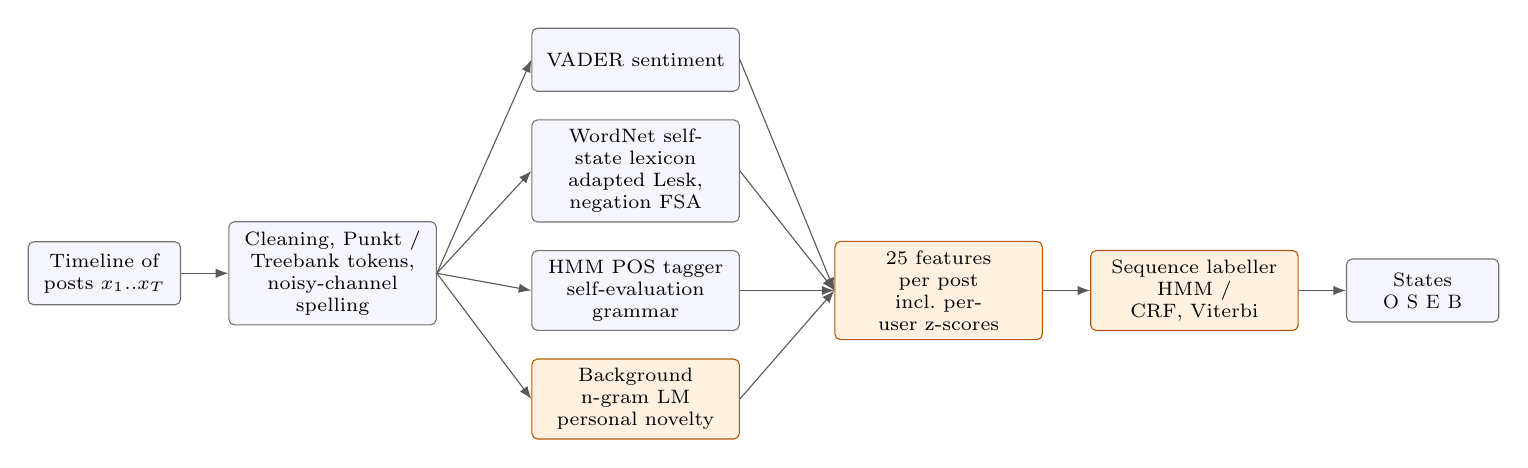
\begin{tikzpicture}[
  node distance=3.5mm and 6mm,
  box/.style={draw=black!55, rounded corners=2pt, align=center, font=\scriptsize, fill=blue!4, minimum height=8mm, text width=24mm},
  hl/.style={box, fill=orange!12, draw=orange!70!black},
  arr/.style={-{Latex[length=1.6mm]}, draw=black!65}]
  \node[box, text width=17mm] (in) {Timeline of\\posts $x_1..x_T$};
  \node[box, right=of in] (norm) {Cleaning, Punkt / Treebank tokens,\\noisy-channel spelling};
  \node[box, right=12mm of norm, yshift=13mm] (lex) {WordNet self-state lexicon\\adapted Lesk, negation FSA};
  \node[box, below=of lex] (pos) {HMM POS tagger\\self-evaluation grammar};
  \node[hl, below=of pos] (lm) {Background n-gram LM\\personal novelty};
  \node[box, above=of lex] (vad) {VADER sentiment};
  \node[hl, right=12mm of pos] (feat) {25 features per post\\incl.\ per-user z-scores};
  \node[hl, right=of feat] (seq) {Sequence labeller\\HMM / CRF, Viterbi};
  \node[box, right=of seq, text width=17mm] (out) {States\\\state{O} \state{S} \state{E} \state{B}};
  \draw[arr] (in) -- (norm);
  \foreach \t in {lex,pos,lm,vad} \draw[arr] (norm.east) -- (\t.west);
  \foreach \t in {lex,pos,lm,vad} \draw[arr] (\t.east) -- (feat.west);
  \draw[arr] (feat) -- (seq);
  \draw[arr] (seq) -- (out);
\end{tikzpicture}}
\caption{The DriftLens pipeline. Every component is a classical NLP method that runs on a CPU. Orange boxes mark the parts that model change relative to the user and over time.}
\label{fig:pipeline}
\end{figure}

Figure~\ref{fig:pipeline} shows the pipeline. Each post is normalised and scored by four label-free components, their outputs become a feature vector, and a sequence model assigns the states. Because nothing before the sequence model sees a CLPsych label, the features can be computed once, outside the cross-validation loop.

\subsection{Normalisation and Noisy-Channel Spelling Correction}

Reddit markup (links, user and subreddit mentions, emphasis) is removed, letters repeated three or more times are shortened to two, and a short list of apostrophe-less contractions (\emph{im}, \emph{dont}, \emph{cant}) is expanded. Sentences and words are segmented with NLTK's Punkt and Treebank tokenisers. For a token $x$ that is not in the dictionary, even after WordNet's inflectional analysis, the corrector chooses
\begin{equation}
\hat{w} = \arg\max_{w \in C(x) \cup \{x\}} \; \log P(w \mid w_{-1}) + \log P(w_{+1} \mid w) - \alpha\, d(x, w),
\end{equation}
where $C(x)$ holds the dictionary words within two edits of $x$ and the language-model terms come from the background bigram model of Sect.~\ref{sec:lm}. Out-of-vocabulary candidates share the probability of the unknown-word token in proportion to their unigram counts; without this step every rare candidate inherits the large probability of \texttt{<unk>}. The channel cost $d$ is a weighted Damerau--Levenshtein distance~\cite{damerau1964technique} in the spirit of Kernighan et al.~\cite{kernighan1990spelling}. It charges 0.5 for substituting a key adjacent on a QWERTY keyboard, 0.7 for swapping two vowels, 0.6 for inserting or deleting a doubled letter and for a transposition, and 1 otherwise. Including the typed word $x$ itself with $d=0$ is the ``no error'' hypothesis. It lets rare slang and names survive unless a correction is clearly more probable.

\subsection{Background Language Model and Personal Novelty}
\label{sec:lm}

The background model is a word bigram model with Jelinek--Mercer interpolation~\cite{jelinek1980interpolated,chen1999empirical},
\begin{equation}
P_{\text{bg}}(w_i \mid w_{i-1}) = \lambda_2\, P_{\text{ML}}(w_i \mid w_{i-1}) + \lambda_1\, P_{\text{add-}k}(w_i),
\end{equation}
trained on 1.5M eRisk tokens (vocabulary 33,372 words with count $\ge 2$), with $\lambda$ tuned on a 60k-token development set. For post $t$ of a user we also train a small add-$k$ bigram model $P_{u,t}$ ($k=0.05$) on the same user's posts $1..t-1$ and mix the two, $P_{\text{mix}} = \beta P_{u,t} + (1-\beta) P_{\text{bg}}$ with $\beta = 0.3$. Personal novelty is the resulting change in cross-entropy, in bits per token:
\begin{equation}
\mathrm{nov}_t = H_{\text{mix}}(x_t) - H_{\text{bg}}(x_t), \qquad H_{P}(x_t) = -\tfrac{1}{|x_t|}\textstyle\sum_i \log_2 P(w_i \mid w_{i-1}).
\end{equation}
When a post reuses the writer's habitual words and phrases, the personal component raises the probabilities and $\mathrm{nov}_t$ is negative. When the post breaks from the writer's past, the personal component only takes probability mass away and $\mathrm{nov}_t$ approaches its upper bound $-\log_2(1-\beta) \approx 0.51$. Subtracting $H_{\text{bg}}$ removes the effect of how predictable the text is in general. We also record the share of a post's content-word types that the user has not used before.

\subsection{WordNet-Grown Self-State Lexicon}

\paragraph{Construction.}
Twelve categories loosely follow the adaptive and maladaptive self-state evidence of CLPsych 2025. The seven maladaptive categories are despair, self-criticism, anxiety, anger, isolation, exhaustion and crisis, and the five adaptive ones are hope, connection, calm, joy and agency. The seeds are 94 WordNet synsets rather than words, so that, for example, the emotional sense \texttt{hopeless.a.01} is kept apart from ``hopeless at maths''. From each seed we follow similar-to, also-see, attribute, derivation, pertainym, verb-group and hyponym links for up to two hops. The weight is multiplied by 0.7--0.85 per hop, and hyponyms must stay within a Wu--Palmer similarity~\cite{wu1994verb} of 0.6 to their seed. Crisis seeds only admit derivational relatives, because their similar-to neighbours drift to generic words such as \emph{dangerous} and \emph{risky}. Antonyms of a seed enter the opposite polarity with weight 0.6.

A word reached this way may still be used mostly in an unrelated sense. We therefore compute its \emph{sense ratio}
\begin{equation}
r(w) = \frac{\sum_{s \in S_{\text{reached}}(w)} \big(c(w,s)+1\big)}{\sum_{s \in S(w)} \big(c(w,s)+1\big)},
\end{equation}
where $S(w)$ contains only synsets that list $w$ itself as a lemma and $c(w,s)$ is the SemCor count WordNet provides. The final weight is the path weight times $\sqrt{r(w)}$, and words with $r(w) < 0.2$ (0.1 for seed lemmas) are dropped. This removes \emph{down}, \emph{blue} and \emph{low}, whose everyday senses are not about mood. Finally, an expanded word is vetoed when SentiWordNet~\cite{esuli2006sentiwordnet} or its VADER valence clearly contradicts the category's polarity (a margin of 0.25 or $|v| \ge 1$). The result has 1,760 words (1,076 maladaptive, 684 adaptive) after 312 vetoes, plus 30 hand-written multi-word expressions such as \emph{end it all} or \emph{reach out} that WordNet cannot supply.

\paragraph{Scoring.}
A token is looked up directly, then after inflectional analysis with WordNet's \texttt{morphy}, and then after a small derivational suffix stripper (\emph{hopelessness} $\rightarrow$ \emph{hopeless}). The 700 lexicon words with $r(w) < 0.7$ are disambiguated in their sentence with an adapted Lesk algorithm~\cite{banerjee2002adapted}. The signature of a sense is the bag of content words in its gloss, examples and lemma names, and in those of its similar-to, hypernym and also-see neighbours. The score is the overlap with the sentence. Senses in the lexicon get one extra point when another affect word appears in the same sentence, a one-domain-per-context cue~\cite{magnini2002role}. Ties go to the more frequent sense. A hit counts only if the chosen sense is one of the reached senses, so ``anxious to see the new film'' is rejected. We adapted Lesk in this way because NLTK's simplified Lesk breaks zero-overlap ties by synset name, which is effectively arbitrary. Negation is a two-state finite-state machine. A cue (\emph{not}, \emph{never}, \emph{n't}, \dots) opens a scope that closes after three words or at a clause boundary. A negated adaptive word counts half towards the maladaptive side (``not happy''), and a negated maladaptive word is dropped, since ``not sad'' does not mean happy. Scores are expressed per 100 words.

\subsection{HMM Tagger and Self-Evaluation Grammar}

The tagger is a bigram HMM over the 12 universal tags, trained on 51,606 Brown sentences with add-$k$ smoothing ($k=0.1$ for transitions, 0.01 for emissions) and decoded with Viterbi. Unknown words follow TnT~\cite{brants2000tnt}. The tag distribution of rare training words that share the longest known suffix (up to four letters) is turned into an emission score by Bayes' rule. When no suffix matches, a shape class (capitalised, digit, hyphenated) is used instead. After tagging, first-person pronouns, copular verbs, auxiliaries and negations receive their own tags, and a cascaded regular grammar chunks clauses such as ``I am so worthless'', ``I don't enjoy'' or ``I hate myself'':
\begin{center}\small
\texttt{SELF $\rightarrow$ FP (ADV|NEG)* (AUX|VERB|COP)* COP (ADV|NEG)* \dots\ (ADJ|VERB|NOUN)}\\
\texttt{SELF $\rightarrow$ FP (ADV|NEG|AUX)* VERB FPO} \qquad \texttt{SELF $\rightarrow$ FP (ADV|NEG|AUX|COP)* VERB}
\end{center}
A chunk counts as a negative or positive self-evaluation according to the lexicon polarity of its words, with a negation inside the chunk flipping adaptive words. The grammar is a finite-state approximation of a small context-free grammar. The prototype also shows the full CFG, its Chomsky normal form, and top-down and bottom-up parses.

\subsection{Post Features}

Table~\ref{tab:features} lists the 25 features. Deltas to the previous and next post are allowed because the task is retrospective: the whole timeline is available, as in CLPsych. The personal group re-expresses six signals as z-scores within the user's own timeline, so that a post is described by how unusual it is \emph{for this writer}.

\begin{table}[t]
\caption{Per-post features. ``Balance'' is the adaptive minus the maladaptive lexicon score.}
\label{tab:features}
\centering\small
\begin{tabular}{@{}lcp{0.78\textwidth}@{}}
\toprule
Group & \# & Features \\
\midrule
LEN   & 1 & log word count \\
LEX   & 8 & maladaptive, adaptive, balance, crisis flag; balance minus the user's running mean, minus the previous post, and next post minus this post; absolute deviation from the running mean \\
SENT  & 3 & VADER compound; its change from the previous and to the next post \\
SELF  & 3 & first-person singular rate; negative and positive self-evaluation chunks \\
DRIFT & 2 & personal LM novelty; share of content words new to this user \\
TIME  & 2 & log days since previous post; first-post indicator \\
PERS  & 6 & within-timeline z-scores of length, maladaptive, balance, VADER, first person, novelty \\
\bottomrule
\end{tabular}
\end{table}

\subsection{Timeline Sequence Models}

Let $\mathbf{x}_{1:T}$ be the feature vectors of a timeline and $y_t \in \{\state{O},\state{S},\state{E},\state{B}\}$ the states. We compare four families that mirror the classical POS-tagging models: independent versus sequential, generative versus conditional.

\emph{MaxEnt} is a multinomial logistic regression~\cite{berger1996maximum} on standardised features with class-balanced weights, fitted with scikit-learn~\cite{pedregosa2011scikit}. It labels each post independently.

\emph{Gaussian HMM} is estimated by supervised maximum likelihood. The initial and transition probabilities are add-one smoothed counts, and each state emits a diagonal Gaussian over the standardised features (variance floor 0.05). Decoding uses Viterbi,
\begin{equation}
\hat{y}_{1:T} = \arg\max_{y_{1:T}} \log \pi_{y_1} + \sum_{t=2}^{T} \log A_{y_{t-1} y_t} + \sum_{t=1}^{T} \log p(\mathbf{x}_t \mid y_t).
\end{equation}

\emph{MaxEnt--HMM hybrid} replaces the Gaussian emission with a scaled likelihood from the MaxEnt classifier~\cite{bourlard1994connectionist}. In the textbook variant this is $p(y \mid \mathbf{x}) / p(y)$ from an unweighted classifier. In the \emph{balanced} variant the classifier is trained with class-balanced weights, so its posterior already behaves as if the prior were uniform and needs no division.

\emph{Linear-chain CRF}~\cite{lafferty2001conditional} is trained with L-BFGS and elastic-net penalties $c_1 = c_2 = 0.1$ using CRFsuite~\cite{okazaki2007crfsuite}. Viterbi decoding of a likelihood-trained CRF favours the majority state. We therefore also use \emph{prior-corrected posterior decoding},
\begin{equation}
\hat{y}_t = \arg\max_{y} \; P(y_t = y \mid \mathbf{x}_{1:T}) \,/\, \pi^{\text{train}}_y,
\end{equation}
where the marginals come from forward--backward. This is the Bayes decision under a uniform state prior, the parameter-free counterpart of class-balanced training.

%======================================================================
\section{Experimental Setup}
%======================================================================

All supervised results use five-fold cross-validation at the \emph{timeline} level, so no user appears in both training and test folds. The procedure is repeated with five different shuffles. Predictions from the five folds are pooled before scoring, and we report the mean and standard deviation over the repetitions. Close to the post-level evaluation of CLPsych 2022, we score three binary views of the four states: switch (\state{S} or \state{B}), escalation (\state{E} or \state{B}) and no change. Macro-F1 is the mean of the three F1 scores. Hyper-parameters are library defaults fixed before any run ($C = 1$ for MaxEnt, $c_1 = c_2 = 0.1$ for the CRF), because 30 timelines are too few for nested tuning. For significance we use a paired bootstrap over timelines~\cite{efron1993introduction,bergkirkpatrick2012empirical}. Each of 1,000 resamples draws 30 timelines with replacement and averages the metric over the five repetitions, so the variation from fold assignment is integrated out.

One caveat about the process should be stated plainly. After a first cross-validation run we added the class-balance corrections and the personal z-scores, and we report the earlier variants next to the final ones. Because no labelled test set remains untouched, the numbers may be slightly optimistic.

%======================================================================
\section{Results}
%======================================================================

\subsection{The Classical Components on Their Own}

\begin{table}[t]
\caption{Intrinsic evaluation of the components. Left: perplexity of language models trained on 1.5M eRisk tokens, measured on the eRisk development set and on all 465 CLPsych posts (61,942 tokens); $k$ and $\lambda$ are tuned on the development set. Right, top: universal-tag accuracy of the taggers; ``unk.'' is the accuracy on words unseen in training. Right, bottom: top-1 accuracy of the spelling corrector on 1,000 synthetic non-word errors in CLPsych words ($\alpha$ tuned on 500 other items).}
\label{tab:components}
\centering\small
\begin{tabular}[t]{@{}llrr@{}}
\toprule
Order & Smoothing & Dev & CLPsych \\
\midrule
1-gram & Laplace          & 825 & 604 \\
       & add-$k$ (0.001)  & 820 & 597 \\
2-gram & Laplace          & 1,788 & 1,335 \\
       & add-$k$ (0.005)  & 403 & 276 \\
       & Jelinek--Mercer  & 254 & 192 \\
3-gram & Laplace          & 10,108 & 10,541 \\
       & add-$k$ (0.001)  & 1,597 & 1,629 \\
       & Jelinek--Mercer  & \textbf{209} & \textbf{176} \\
\bottomrule
\end{tabular}\hfill
\begin{tabular}[t]{@{}lrr@{}}
\toprule
Tagger (test set) & Acc. & Unk. \\
\midrule
HMM, ours (Brown)          & \textbf{96.9} & 82.7 \\
HMM, ours (Treebank)       & 88.9 & 61.3 \\
NLTK perceptron (Brown)    & 92.0 & -- \\
NLTK perceptron (Treebank) & 96.1 & -- \\
\midrule
Spelling channel and prior & \multicolumn{2}{r}{Acc.} \\
\midrule
Levenshtein + unigram      & \multicolumn{2}{r}{88.8} \\
Weighted + unigram         & \multicolumn{2}{r}{90.7} \\
Weighted + bigram context  & \multicolumn{2}{r}{\textbf{95.3}} \\
\quad + ``no error'' option & \multicolumn{2}{r}{94.1} \\
\bottomrule
\end{tabular}
\end{table}

Table~\ref{tab:components} summarises the components. The language models reproduce the classic lesson on smoothing: add-one smoothing gives so much mass to unseen events that a trigram model becomes worse than a unigram model (perplexity 10,541 vs.\ 604). Interpolation gives the lowest perplexity, 176 for the trigram. The CLPsych posts are, if anything, easier than the eRisk development text, which suggests that the background model transfers across the two Reddit collections.

Our HMM tagger reaches 96.9\% on held-out Brown sentences. On the Treebank sample it drops to 88.9\%, partly because of the domain shift and partly because the Brown and Penn tag sets map onto the universal tags in slightly different ways. NLTK's perceptron tagger shows the mirror image, since it was trained on Wall Street Journal text. Each tagger is best in its own domain.

For spelling, the keyboard-weighted channel helps most on adjacent-key substitutions (97\% vs.\ 90\%), and bigram context helps most on deletions (84\% vs.\ 66--69\%), where many candidates are equally close. The ``no error'' option costs 1.2 points on synthetic errors, but it matters on real text. Of the 341 out-of-dictionary tokens in CLPsych, it rewrites 63\%, while forced correction rewrites 89\%, most of the difference being slang and names.

\subsection{Is the Lexicon Measuring Self-State?}

\begin{figure}[t]
\centering
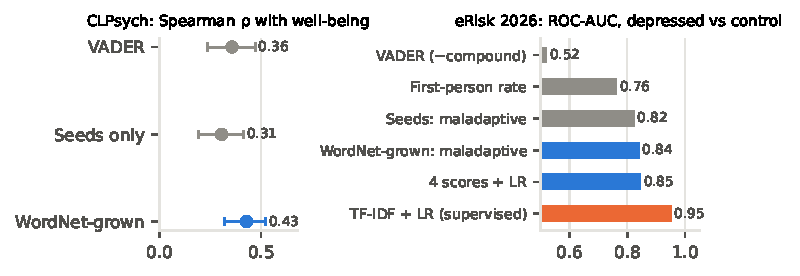
\includegraphics[width=\textwidth]{fig_lexicon}
\caption{Validity of the lexicon. Left: Spearman correlation between the post-level balance score and the annotated 1--10 well-being rating (236 posts, 95\% bootstrap intervals). Right: ROC-AUC for separating the 102 depressed from the 807 control users of eRisk 2026, using each user's last 100 writings. Only the orange bar uses training labels.}
\label{fig:lexicon}
\end{figure}

Figure~\ref{fig:lexicon} shows two independent checks. On CLPsych, the balance score of the WordNet-grown lexicon correlates with the annotated well-being rating at $\rho = 0.43$ [0.32, 0.52], compared with 0.31 for the seed lemmas alone and 0.36 for VADER. Post length is unrelated to well-being ($\rho = -0.06$), so this is not a length artefact. Almost all of the signal sits on the maladaptive side ($\rho = -0.47$), and the adaptive score is uncorrelated with well-being ($\rho = -0.01$). Against the annotated evidence, the lexicon finds at least one maladaptive hit inside 39\% of the 615 maladaptive spans (seeds: 31\%), and 38\% of its maladaptive hits fall inside such a span. Adaptive evidence is harder: 27\% recall at 25\% precision.

On eRisk, the maladaptive density of a user's writings separates depressed from control users with an AUC of 0.84 (seeds: 0.82) without seeing a single label. First-person pronoun rate gives 0.76, a replication of Rude et al.~\cite{rude2004language}, while the VADER compound is at chance (0.52). The adaptive score points the \emph{other} way: depressed users use more adaptive words (AUC 0.69 for the adaptive score), probably because they write in support communities where words like \emph{therapy}, \emph{friends} and \emph{hope} are frequent. A supervised TF-IDF classifier is much stronger (AUC 0.95), which is expected, because it can learn topics and community vocabulary. The value of the lexicon is that it needs no labels and every hit can be explained.

Three components had no measurable effect on these aggregate scores: WSD, negation handling and spelling correction each moved $\rho$ by at most 0.012. They make individual highlights more trustworthy in the prototype, but we cannot claim that they improve the numbers.

\subsection{Detecting Moments of Change}

\begin{table}[t]
\caption{Moment-of-change detection on the 30 CLPsych training timelines (373 posts), 5 repetitions of 5-fold timeline-level cross-validation. Mean $\pm$ standard deviation over repetitions.}
\label{tab:main}
\centering\small
\begin{tabular}{@{}lccc@{}}
\toprule
System & Macro-F1 & F1 switch & F1 escalation \\
\midrule
Majority (all \state{O})             & 0.266 $\pm$ .000 & 0.000 & 0.000 \\
MaxEnt, post length only             & \textbf{0.572} $\pm$ .008 & 0.483 & 0.470 \\
\midrule
MaxEnt (independent posts)           & 0.547 $\pm$ .002 & 0.476 & 0.420 \\
Gaussian HMM                         & 0.567 $\pm$ .008 & \textbf{0.508} & 0.469 \\
MaxEnt--HMM hybrid, prior-divided    & 0.542 $\pm$ .005 & 0.357 & 0.471 \\
MaxEnt--HMM hybrid, balanced         & 0.532 $\pm$ .013 & 0.335 & 0.467 \\
CRF, Viterbi                         & 0.533 $\pm$ .011 & 0.374 & 0.416 \\
CRF, prior-corrected                 & 0.563 $\pm$ .008 & 0.472 & \textbf{0.481} \\
\bottomrule
\end{tabular}
\end{table}

\begin{figure}[t]
\centering
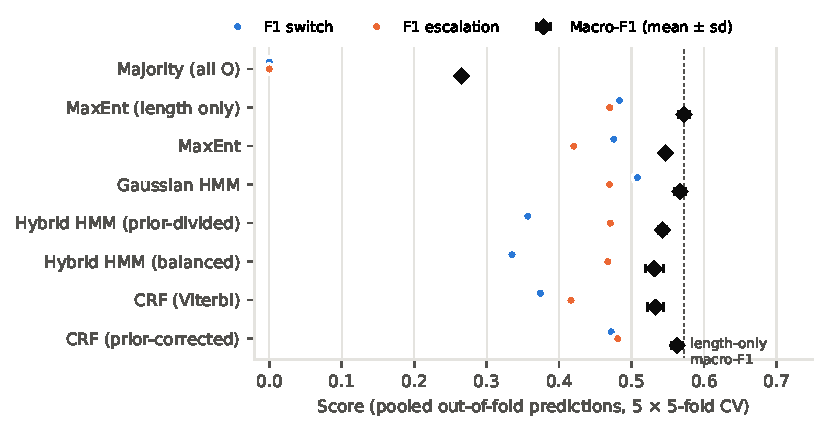
\includegraphics[width=0.92\textwidth]{fig_models}
\caption{Per-model scores from Table~\ref{tab:main}. The dotted line marks the macro-F1 of the length-only classifier.}
\label{fig:models}
\end{figure}

Table~\ref{tab:main} and Fig.~\ref{fig:models} give the main results. All models are far above the majority baseline (for the HMM, bootstrap $p < 0.001$). The Gaussian HMM has the best macro-F1 among the full-feature models (0.567) and the best switch F1 (0.508). The prior-corrected CRF has the best escalation F1 (0.481). Against the per-post MaxEnt, the HMM gains 0.049 escalation F1 ($p = 0.086$) and 0.032 switch F1 ($p = 0.087$). These differences are consistent across repetitions but do not reach the 5\% level with 30 timelines. The class-balance fix matters for the CRF: prior-corrected decoding raises its macro-F1 from 0.533 to 0.563 and its switch F1 from 0.374 to 0.472. For the hybrid HMM, balancing the classifier did not help, and the textbook prior division was slightly better.

The most important row is the second one. A logistic regression that sees nothing but the logarithm of the post length reaches 0.572, and neither the HMM ($-0.006$, $p = 0.60$) nor the CRF ($-0.010$, $p = 0.67$) beats it. Change posts are simply much longer: the median switch or escalation post has about 150 words, the median unchanged post about 20 (Mann--Whitney $p < 10^{-19}$). People seem to write at length when something has happened, so length is a real signal, but it is also a shortcut in the sense of Geirhos et al.~\cite{geirhos2020shortcut}. A model that relies on it would miss a short, bleak post and flag every long, cheerful one.

\begin{table}[t]
\caption{Macro-F1 within length strata (split at the median, 46 words), mean over 5 repetitions. Within a stratum, length carries little information and the linguistic features must do the work.}
\label{tab:strata}
\centering\small
\begin{tabular}{@{}lcc@{}}
\toprule
System & Short posts ($\le$ 46 words) & Long posts ($>$ 46 words) \\
\midrule
MaxEnt, post length only & 0.311 & 0.369 \\
MaxEnt, all features     & 0.393 & 0.463 \\
Gaussian HMM             & 0.373 & 0.413 \\
CRF, prior-corrected     & \textbf{0.404} & \textbf{0.495} \\
\bottomrule
\end{tabular}
\end{table}

Table~\ref{tab:strata} separates the two effects. Within posts of similar length, the length-only model falls to 0.31 and 0.37, while the CRF with all features reaches 0.40 and 0.50, a gain of 0.09 and 0.13. The overall tie between the models therefore hides a real contribution of the linguistic features. Length explains \emph{which half} of the data a post falls into, and the features explain which posts \emph{within} each half are moments of change. The HMM is weaker here than its overall score suggests. A likely reason is that its diagonal Gaussian emissions produce very confident posteriors, which exploit the length split well but leave little room for finer distinctions within a stratum.

\subsection{What the Features Contribute}

\begin{figure}[t]
\centering
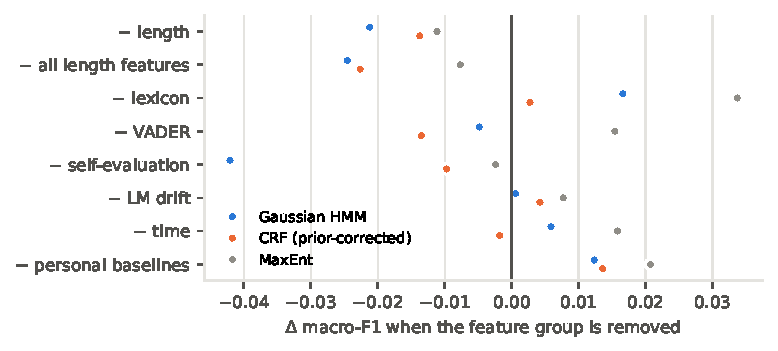
\includegraphics[width=0.92\textwidth]{fig_ablation}
\caption{Change in cross-validated macro-F1 when one feature group is removed (full models: HMM 0.567, CRF 0.563, MaxEnt 0.547). Negative values mean the group helps.}
\label{fig:ablation}
\end{figure}

Figure~\ref{fig:ablation} removes one feature group at a time. The self-evaluation features from the tagger and grammar are the most useful non-length group for the HMM ($-0.042$), and VADER helps the CRF ($-0.014$). Removing the lexicon group slightly \emph{improves} all three models (+0.003 to +0.034), and the same holds for the personal z-scores. With 373 posts and 25 features, redundant groups add variance: the lexicon balance and VADER are correlated, and the z-scores repeat information that the running-mean deltas already carry. The lexicon still matters in another way. Building the features from the seed lemmas instead of the grown lexicon lowers the HMM from 0.567 to 0.547. Used alone, the drift group reaches 0.474 with the HMM but only 0.389 with MaxEnt, and the personal group alone reaches 0.533 and 0.515. Signals defined relative to the user therefore carry much of the information on their own (although the vocabulary share in the drift group is partly a length effect, as shown below), even though they add little on top of the other groups.

\begin{figure}[t]
\centering
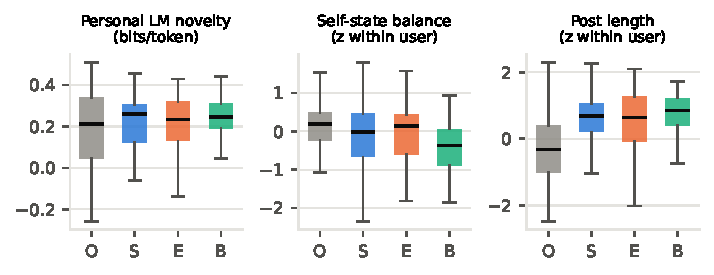
\includegraphics[width=0.9\textwidth]{fig_signals}\\[2mm]
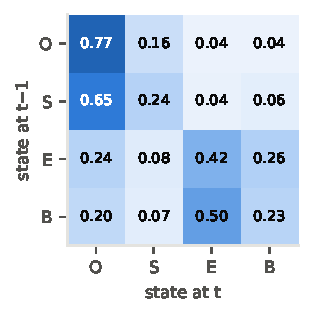
\includegraphics[width=0.4\textwidth]{fig_transitions}
\caption{Top: distribution of three signals by gold state (first posts excluded). Bottom: transition matrix of the Gaussian HMM trained on all 30 timelines. Escalation persists ($\state{E}\!\to\!\state{E}$ 0.42, $\state{B}\!\to\!\state{E}$ 0.50), while a switch is usually followed by no change (0.65).}
\label{fig:signals}
\end{figure}

Figure~\ref{fig:signals} shows why the sequence models help on escalation. The learned transitions keep an escalation going for several posts, while a switch is almost always followed by a return to \state{O}. The signals behave as expected, with one exception. The balance score is lower for change posts (median $-0.91$ for \state{E} and $-1.14$ for \state{B} against 0.00 for \state{O}, $p < 10^{-4}$), and its absolute deviation from the user's running mean is larger ($p < 0.001$). VADER separates the two kinds of change: switch posts have a \emph{positive} median compound score (+0.46), because many switches are sudden improvements, while escalation posts are negative ($-0.68$). The exception is personal LM novelty. Its median is higher for switch posts than for unchanged posts (0.26 vs.\ 0.21 bits per token), but change posts as a whole do not differ significantly from unchanged ones (Mann--Whitney $p = 0.25$). The share of new vocabulary is significant, but it goes down for change posts, which is a side effect of length (long posts repeat more of their own words). The idea that a changing person starts to sound unlike themselves is attractive, but a word-bigram model trained on a dozen posts is too weak to show it reliably.

\begin{figure}[t]
\centering
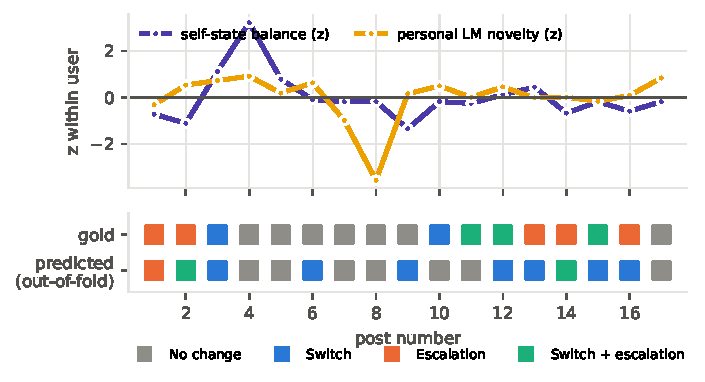
\includegraphics[width=0.85\textwidth]{fig_example}
\caption{One training timeline (17 posts) with its out-of-fold CRF predictions. The model finds the opening escalation and the switch at post 3, raises two false switches (posts 6 and 9), and labels most of the late escalation run (posts 11--16) as switches. Text is not shown for privacy.}
\label{fig:example}
\end{figure}

Figure~\ref{fig:example} shows a typical timeline. The model finds the opening escalation and the first switch, but it labels the late escalation run as a series of switches. Telling an abrupt change from a gradual one requires a notion of trend that our pairwise deltas only approximate.

%======================================================================
\section{The Prototype}
%======================================================================

The prototype is a Streamlit application that runs on a laptop CPU and loads all models in under a second. A user can paste their own posts or choose a CLPsych timeline. The main view plots the balance score, VADER and personal novelty over the timeline, with coloured bands for the predicted and gold states. Every post opens to show its text with maladaptive, adaptive, crisis and negated words highlighted, the extracted self-evaluations, the spelling corrections, its signals and the state probabilities. A digest tab summarises the timeline with TextRank~\cite{mihalcea2004textrank}, whose teleport vector is biased towards sentences containing self-state words, as in topic-sensitive PageRank~\cite{haveliwala2002topic}. The digest is not evaluated. A toolbox tab gives one interactive panel per technique: the candidate table of the noisy channel, per-token bigram probabilities and a live novelty calculation, the HMM and perceptron tags side by side with the chunk tree and top-down and bottom-up CFG parses, and a WordNet panel with synsets, path, Wu--Palmer, Leacock--Chodorow, Resnik~\cite{resnik1995using}, Lin~\cite{lin1998information} and Jiang--Conrath similarities, and both Lesk variants. For deployment we use the prior-corrected CRF. Its cross-validated score is within noise of the HMM, and its probabilities are better calibrated, whereas the HMM's saturate near 0 or 1.

%======================================================================
\section{Limitations and Ethical Considerations}
%======================================================================

The evaluation rests on 30 labelled timelines. Differences of 0.02 macro-F1 are within the noise, and several design choices were made after a first cross-validation run, so the absolute numbers may be optimistic. The labels are subjective, and the lexicon categories are our reading of the CLPsych self-state framework, not the official taxonomy. The seed synsets were chosen by us; a different set might change the lexicon results. The personal novelty score did not work as hoped, possibly because the per-user models are trained on very little text. Finally, all data are English Reddit posts. A transfer to code-mixed Hindi--English would need new resources at every stage.

A system that labels a person's mental state from their posts can harm them if it is wrong or misused. DriftLens is a research prototype, not a diagnostic or monitoring tool. It shows its evidence precisely so that a human can disagree with it. It should never be used to make decisions about individuals. The prototype displays the Indian Tele-MANAS helpline (14416) for anyone who needs support.

%======================================================================
\section{Conclusion}
%======================================================================

Reading a timeline as a sentence works in the sense one would hope: an HMM or CRF over carefully built classical features detects moments of change far better than chance, and sequence structure helps most where the labels come in runs, on escalation. The more useful lesson is about evaluation. On this dataset post length alone matches every model we built, and only a length-stratified analysis reveals that the linguistic features add 0.09 to 0.13 macro-F1 within comparable posts. Along the way, the WordNet-grown lexicon proved a better measure of self-state than a general sentiment tool, both against well-being ratings and, without labels, on an external depression corpus. Next steps are trend features over windows of posts, which should help separate escalation from switches, and personal language models with character n-grams or backoff to similar users, so that the drift idea gets a fairer test.

\subsubsection*{Acknowledgements.}
We thank the CLPsych and eRisk organisers for access to their data.

\bibliographystyle{splncs04}
\bibliography{references}

\end{document}
